\documentclass[12pt]{article}

% Fonte com acentos
\usepackage[brazil]{babel} \usepackage[utf8]{inputenc} \usepackage[T1]{fontenc}
\usepackage[lighttt]{lmodern} \usepackage[top=1.4in, bottom=1in, left=1in,
right=1in]{geometry} \usepackage{graphicx} % para adicionar imagem
\usepackage{listings} \usepackage{amsmath} \usepackage{indentfirst}

\begin{document}

\setlength{\parskip}{0.2cm}

\title{Análise de código e eficiência do método do Gradiente}

\author{Aryane Ast dos Santos\\ Kevin Katzer}

\date{23 de novembro de 2014}

\maketitle

\tableofcontents

\pagebreak

\section{Introdução}
Motivação...

\section{Verificação de uso de memória com Valgrind}\label{sec:Valgrind}

Ao executar a ferramenta Valgrind para se obter informações sobre vazamento de
memória no programa gradSolver, foi possível observar 5 erros, todos em
contextos diferentes, além de 16 allocações e apenas 2 liberações de memória.

Os resultados da execução do programa são parcialmente apresentados na
figura~\ref{fig:valgrindOut}.

\begin{figure}[htb]
\begin{tt}\noindent
==29599== Command: ./gradSolver -r 5\\
==28949== HEAP SUMMARY:\\
==28949==     in use at exit: 560 bytes in 14 blocks\\
==28949==   total heap usage: 16 allocs, 2 frees, 800 bytes allocated\\
==28949== LEAK SUMMARY:\\
==28949==    definitely lost: 560 bytes in 14 blocks\\
==28949== ERROR SUMMARY: 5 errors from 5 contexts (suppressed: 0 from 0)
\end{tt}\caption{Saída do Valgrind}\label{fig:valgrindOut}
\end{figure}

Aqui o gradSolver foi executado com uma matriz quadrada de ordem 5, porém os
mesmos problemas listados na figura~\ref{fig:valgrindOut} são encontrados em
execuções de matrizes de qualquer dimensão. E de maneira análoga, ao resolver os
problemas apresentados, numa execução com matriz maior, eles ficam também
automaticamente resolvidos.

Para contornar os vazamentos de memória encontrados, foi necessário liberar a
memória dos vetores alocados explicitamente como o vetor x na função main, o
vetor aux em calcGrad e o vetor r de resíduo na função gradSolver. Além disso,
no main, foram adicionados frees para os ponteiros para char das flags do
getopt.

\section{Arquitetura do computador}\label{sec:likwid}

Utilizando a ferramenta likwid-topology, é possível obter as seguintes
informações sobre a arquitetura do computador utilizado para os testes de
performance.

\begin{figure}[ht]\footnotesize
\begin{verbatim}
CPU type:	AMD Magny Cours processor
Hardware Thread Topology
Sockets:	4 
Cores per socket:	8 
Threads per core:	1 
Socket 0: ( 0 1 2 3 4 5 6 7 )
Socket 1: ( 8 9 10 11 12 13 14 15 )
Socket 2: ( 16 17 18 19 20 21 22 23 )
Socket 3: ( 24 25 26 27 28 29 30 31 )
Cache Topology
Level:	1
Size:	64 kB
Cache groups:	( 0 ) ( 1 ) ( 2 ) ( 3 ) ( 4 ) ( 5 ) ( 6 ) ( 7 ) ( 8 ) ( 9 ) ( 10 ) ( 11 ) ( 12 ) ( 13 ) ( 14 ) ( 15 ) ( 16 ) ( 17 ) ( 18 ) ( 19 ) ( 20 ) ( 21 ) ( 22 ) ( 23 ) ( 24 ) ( 25 ) ( 26 ) ( 27 ) ( 28 ) ( 29 ) ( 30 ) ( 31 )
Level:	2
Size:	512 kB
Cache groups:	( 0 ) ( 1 ) ( 2 ) ( 3 ) ( 4 ) ( 5 ) ( 6 ) ( 7 ) ( 8 ) ( 9 ) ( 10 ) ( 11 ) ( 12 ) ( 13 ) ( 14 ) ( 15 ) ( 16 ) ( 17 ) ( 18 ) ( 19 ) ( 20 ) ( 21 ) ( 22 ) ( 23 ) ( 24 ) ( 25 ) ( 26 ) ( 27 ) ( 28 ) ( 29 ) ( 30 ) ( 31 )
Level:	3
Size:	5 MB
Cache groups:	( 0 1 2 3 ) ( 4 5 6 7 ) ( 8 9 10 11 ) ( 12 13 14 15 ) ( 16 17 18 19 ) ( 20 21 22 23 ) ( 24 25 26 27 ) ( 28 29 30 31 )
NUMA Topology
NUMA domains: 8 
Domain 0:
Processors:  0 1 2 3
Relative distance to nodes:  10 16 16 22 16 22 16 22
Memory: 10269.2 MB free of total 16047.3 MB
Cache Topology
Level:	1
Size:	64 kB
Type:	Data cache
Associativity:	2
Number of sets:	512
Cache line size:64
Non Inclusive cache
Shared among 1 threads
Level:	2
Size:	512 kB
Type:	Unified cache
Associativity:	16
Number of sets:	512
Cache line size:64
Non Inclusive cache\
Shared among 1 threads
Level:	3
Size:	5 MB
Type:	Unified cache
Associativity:	96
Number of sets:	512
Cache line size:64
Non Inclusive cache
Shared among 4 threads
\end{verbatim}\caption{Saída do likwid-topology}\label{fig:topologyOut}
\end{figure}

Como pode-se notar na figura~\ref{fig:topologyOut}, nas servidoras do DInf, há
uma CPU Magny Cours, fabricada pela AMD, com 4 socket e 32 cores (8 por socket).

Existem 3 níveis de cache, sendo o primeiro (L1) com 16kB de memória, o segundo
(L2) com 512kB e o terceiro (L3) com 5MB. As caches L1 e L2 são separadas em 32
grupos, sendo que cada grupo é destinado a um core diferente, e o último nível
de cache, L3, é separado em 8 grupos, cada grupo destinado a 4 cores.

Há 8 domínios NUMA, e cada domínio correspondendo a uma cache L3. Como apenas o
Socket 0 será usado, apenas o primeiro domínio NUMA é de interesse para análise
de memória disponivel. O domínio 0 possui 16047.3MB de memória RAM, e no momento
de execução do likwid-topology, havia 10269.2MB de memória livre.

Dada a especificação acima, o maior sistema linear passível de ser resolvido
pela arquitetura descrita é aproximadamente 36600, pois, dada a memória RAM
disponível, e sabendo que o programa aloca $n^2 + 3n$ doubles, temos que $64(n^2 +
3n) = 10269.2\times2^{23}$.

\section{Comparação de desempenho geral}\label{sec:desempenhoGeral}

Para a execução dos testes de desempenho, foi utilizada a ferramenta likwid-pin,
que afixa a execução do programa à um core da máquina em uso dedicado. Mas como
as caches continuam sendo compartilhadas, o que é possível notar na figura
(likwid-topology -g), analisar o desempenho de diferentes execuções se torna um
problema, pois é necessário minimizar o uso de cache pelos outros programas. A
solução encontrada foi executar o gradSolver em single user mode.

No gráfico~\ref{fig:execucao}, é mostrado os tempos de execução em segundos, que
foram obtidos com a função timestamp, para matrizes de dimensões 32, 33, 256,
257, 1024, 1025, 2048 e 2049. O eixo x está em escala logarítmica.

Pode-se notar que na escala do gráfico, as diferenças de tempo de execução entre
os pares de dimensões 32 e 33, 256 e 257, 1024 e 1025, e finalmente 2048 e 2049
são desprezíveis. As execuções do gradSolver com matrizes de dimensões que não
são potência de 2 são ligeiramente melhores, por causa da associatividade da
cache. Uma melhor visualização dos tempos de execução pode ser observada na
tabela~\ref{fig:tabelaExecucoes}.

\begin{figure}[htb]
\begin{tt}\noindent
    32      0.00001764297485352\\
    33      0.00001815387180873\\
    256     0.00094001633780343\\
    257     0.00092514355977376\\
    1024    0.01497772761753627\\
    2048    0.05953870500837054\\
    2049    0.05932899883815220\\
\end{tt}\caption{Tempo de execução por dimensão da matriz}\label{fig:tabelaExecucoes}
\end{figure}

\begin{figure}[htb] \begin{center}
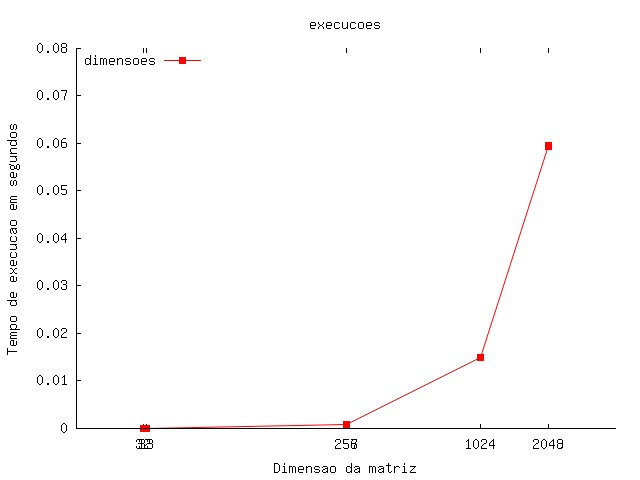
\includegraphics[width=150mm]{execucoes.jpg} \end{center}
\caption{Tempo de execução por dimensão da matriz}\label{fig:execucao}
\end{figure}

\section{Análise do cálculo do fator lambda}\label{sec:lambda}
\subsection{flop operations}
\subsection{mem utilization}
\subsection{explicar graficos flops\_dp, cache, mem}
\subsection{melhoria}

\section{Análise do cálculo do resíduo}\label{sec:residuo}
\subsection{flop operations}
\subsection{mem utilization}
\subsection{explicar graficos flops\_dp, cache, mem}
\subsection{melhoria}

\end{document}
